Схема экспериментальной установки изображена на рис. \ref{pic3}. Для опыта
используется серийная лампа ионизационного манометра ЛМ-$2$, заполненная гелием
до давления $\approx 1$ Торр. Источником электронов является вольфрамовый катод,
нагреваемый переменным током. Напряжение накала подается от стабилизируемого
источника питания С. Ток накала контролируется амперметром А.

\begin{figure}[h]
  \center
  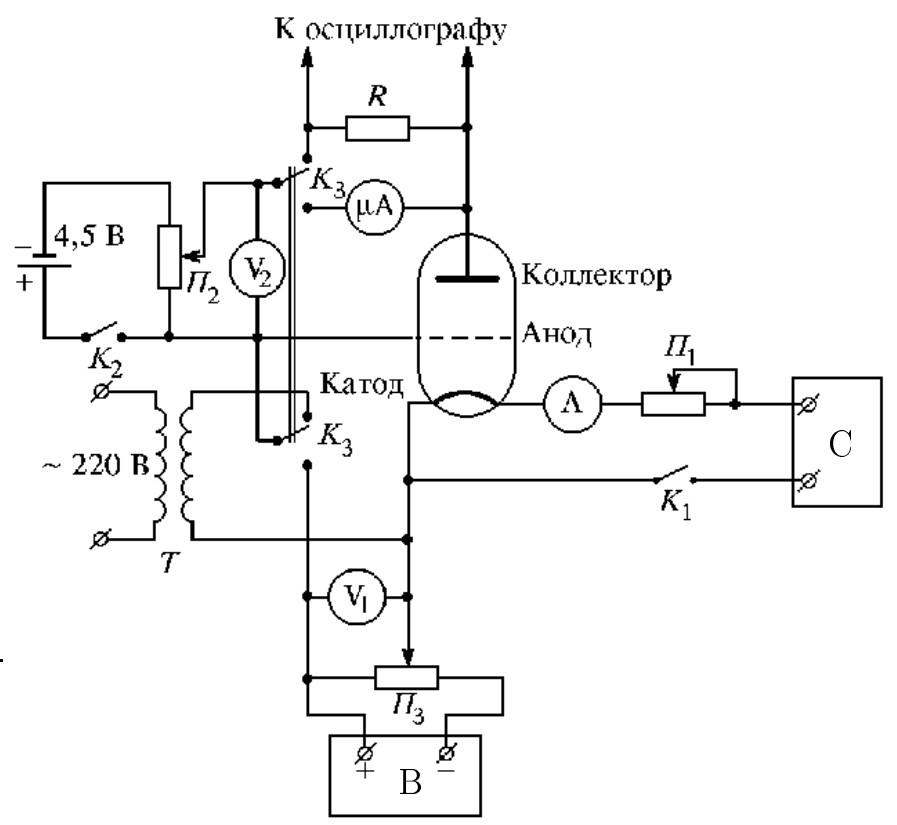
\includegraphics[width=0.8\linewidth]{pic3.png}
  \caption{ Схема экспериментальной установки }
  \label{pic3}
\end{figure}

В качестве анода используется двойная спираль, окружающая катод. Роль коллектора
играет полный металлический цилиндр, соосный с катодом и анодом.

Ускоряющее напряжение подаётся на анод от выпрямителя В. Величина этого
напряжения регулируется потенциометром $\text{П}_3$ и измеряется вольтметром
$V_1$.

Источник задерживающего напряжения -- батарея $4.5$ В; величина напряжения
регулируется потенциометром $\text{П}_2$ и измеряется вольтметром $V_2$. Ток в
цепи коллектора регистрируется микроамперметром.

Схему можно переключать из статического режима измерений в динамический режим с
помощью ключа $\text{К}_3$. На рис. \ref{pic3} две части сдвоенного ключа
$\text{К}_3$ изображены отдельно. При динамическом режиме работы ускоряющий
потенциал подаётся с понижающего трансформатора Т ($220/50$ В), а ток коллектора
регистрируется осциллографом, подключённым к нагрузочному резистору $R$.

При определении энергии электронов по разности потенциалов между анодом и
катодом следует иметь в виду, что из-за контактной разности потенциалов между
катодом и анодом первый максимум не соответствует потенциалу первого
возбуждённого уровня. Однако контактная разность потенциалов сдвигает все
максимумы одинаково, так что расстояние между ними не меняется.

Схема экспериментальной установки, изображенной на рис. \ref{pic3}, в нашей
работе конструктивно осуществлена следующим образом. Наполненная гелием лампа
ЛМ-$2$ расположена непосредственно на корпусе блока источников питания(БИП).
Напряжение к электродам лампы подводится от источников питания, находящихся в
корпусе прибора. Регулировка напряжения и выбор режима работы производится при
помощи ручек управления, выведенных на лицевую панель БИП (рис. \ref{pic4}).
Включение всех источников питания осуществляется включением БИП в сеть.

В статическом режиме напряжение $V_a$ между анодом и катодом измеряется цифровым
вольтметром В$7$-$22$А, подключенным к клеммам <<Вольтметр>> прибора. Ток
коллектора $I_K$ измеряется микроамперметром, вся шкала которого соответствует
току $100$ мкА.

\begin{figure}[h]
  \center
  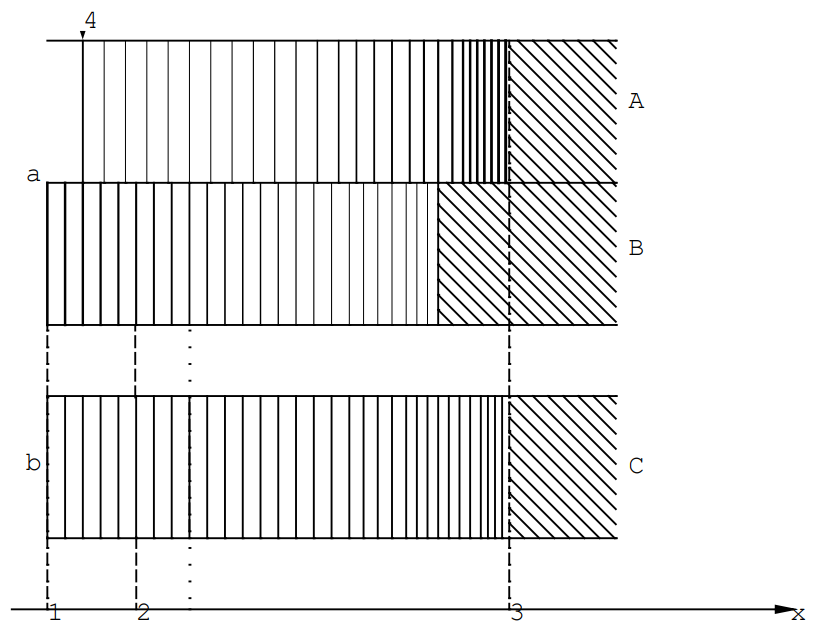
\includegraphics[width=\linewidth]{pic4.png}
  \caption{ Блок-схема экспериментальной установки }
  \label{pic4}
\end{figure}
